\documentclass{standalone}

\usepackage{tikz}
\usetikzlibrary{calc}

\begin{document}

\begin{tikzpicture}
    \def\sqwi{0.6}
   \begin{scope}[local bounding box = scope1] 
        \node at (0,0) {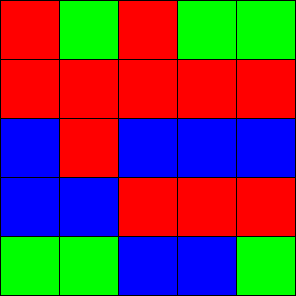
\includegraphics[width=.2\textwidth]{../swap/swap_1.pdf}}; 
        \node at (0.0, -1.75) {labeling $f$};
   \end{scope}
    \begin{scope}[xshift = 5cm, yshift=1cm, transform canvas={scale=0.3}]
               \fill[color=black] (1,0) --(3,0) --(3,1) --(4.5,-1) -- (3,-3) -- (3, -2) -- (1,-2);
    \end{scope}
    \begin{scope}[xshift = 4.5cm]
        \node at (0,0) {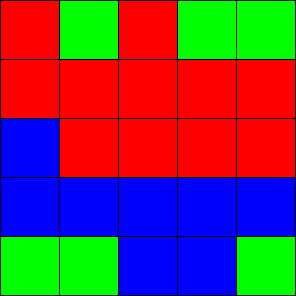
\includegraphics[width=.2\textwidth]{../swap/swap_2.pdf}};
        \node at (0.0, -1.75) {labeling $\hat f$};
    \end{scope}
\end{tikzpicture}

\end{document}
